
\section{Partial Equilibrium Results}




\subsection{Consumption Response to an Increase in Unemployment in Partial Equilibrium}

In this section, I show in partial equilibrium that the aggregate consumption response to a transitory increase in the unemployment rate is deeply persistent in the presence of scarring. I simulate the consumption response to a transitory $1\%$ increase in the unemployment rate in $t=0$. To capture the effects of scarring on consumption, I compare the simulated path of consumption in the baseline model to the simulated path of consumption to a version of the model where scarring is eliminated. I eliminate scarring by setting the probability of human capital accumulation $\pi_{L}$ and the probability of human capital erosion $\pi_{U}$ to zero. Figure \ref{Micro_results} plots the simulated path of consumption to this experiment with and without scarring. Even with $55\%$ of the increase in unemployment rate accounted for by permanent layoffs who are subject to scarring, the response of consumption is significantly more persistent than the response of the unemployment rate. 



\begin{figure}[!ht]
    \centering
   \begin{minipage}{0.49\textwidth}
        \centering
        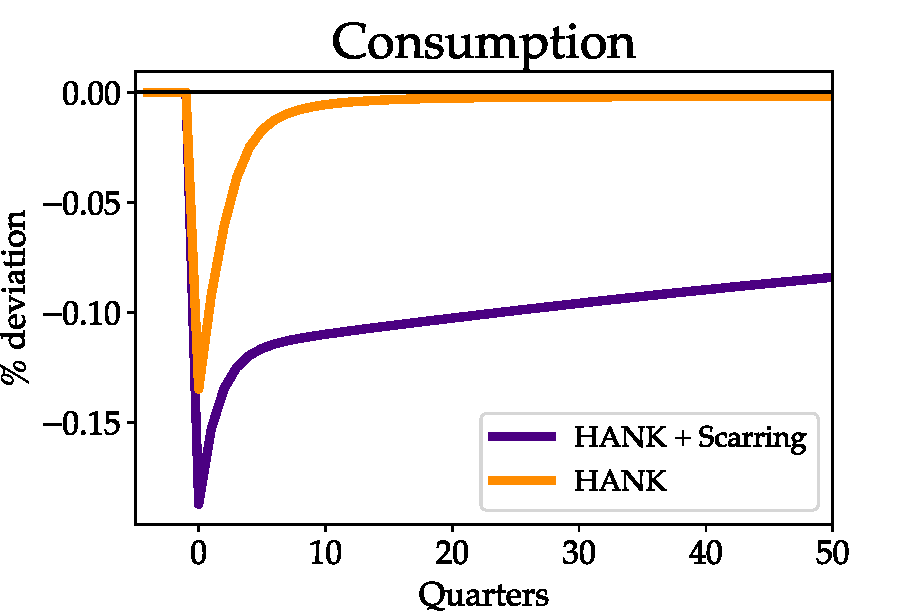
\includegraphics[width=1.1\textwidth]{text/chapter1/Figures/CJAC_JF_real_comparison} 
    \end{minipage}\hfill
    \begin{minipage}{0.49\textwidth}
        \centering
        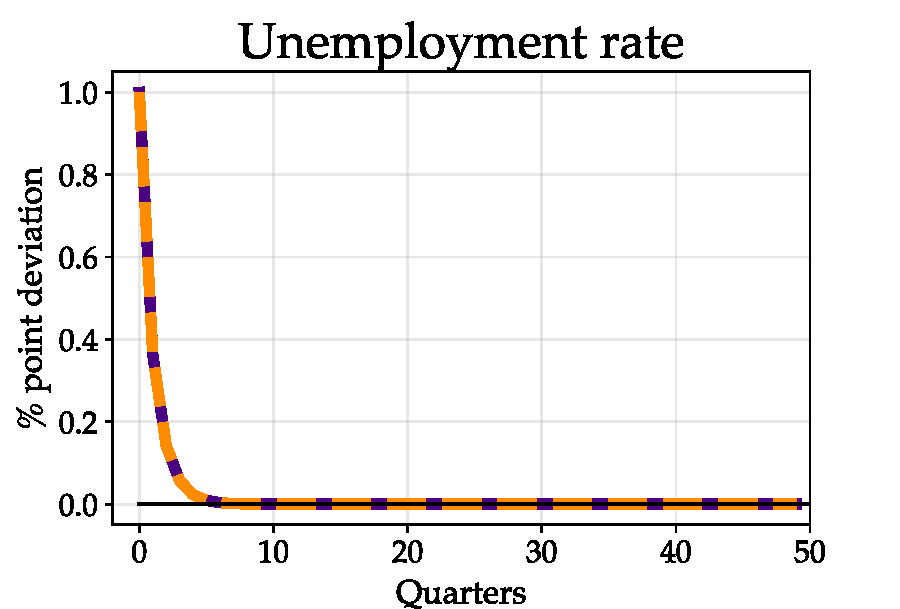
\includegraphics[width=1.1\textwidth]{text/chapter1/Figures/Urate_response_PE}
    \end{minipage}
    \caption{Consumption response to a transitory increase in the unemployment rate}
        \floatfoot{Note: The exercise above plots the consumption response to a one time negative shock to the job finding probability in $t=0$. The size of the one time shock is calibrated to increase the unemployment rate by one percentage point on impact.}
    \label{Micro_results}
\end{figure}





\section{Business Cycle Implications}


\subsection{Macroeconomic Hysteresis}

In this section, I show that unemployment scarring generates hysteresis in macroeconomic fluctuations. To illustrate this, I solve for the impulse responses to a negative demand shock, modeled as a positive discount factor shock. For simplicity, the size of the shock is the same for all ex-ante discount factor groups. The impulse responses to key aggregate variables is plotted in figure \ref{IPR_demand}. In response to this demand shock, increased patience reduces aggregate consumption leading to decreases in output and labor demand. As a result, firms post less vacancies lowering the job finding probability and raising the unemployment rate. As households lose their jobs, on average, they find jobs at a lower wage leading to persistent losses in mean human capital. This causes consumption, output, and labor income to exhibit hysteresis while the unemployment rate recovers with the demand shock. Notably, the responses to consumption, output, debt, and mean human capital still do not recover after 100 quarters, long after the recovery in the unemployment rate. Since unemployment does not exhibit hysteresis, wages nor the vacancy filling rate will either. As a result marginal costs, and therefore inflation, do not exhibit any persistence. 


\begin{figure}[htb]
    \centering % <-- added
\begin{minipage}{0.33\textwidth}
  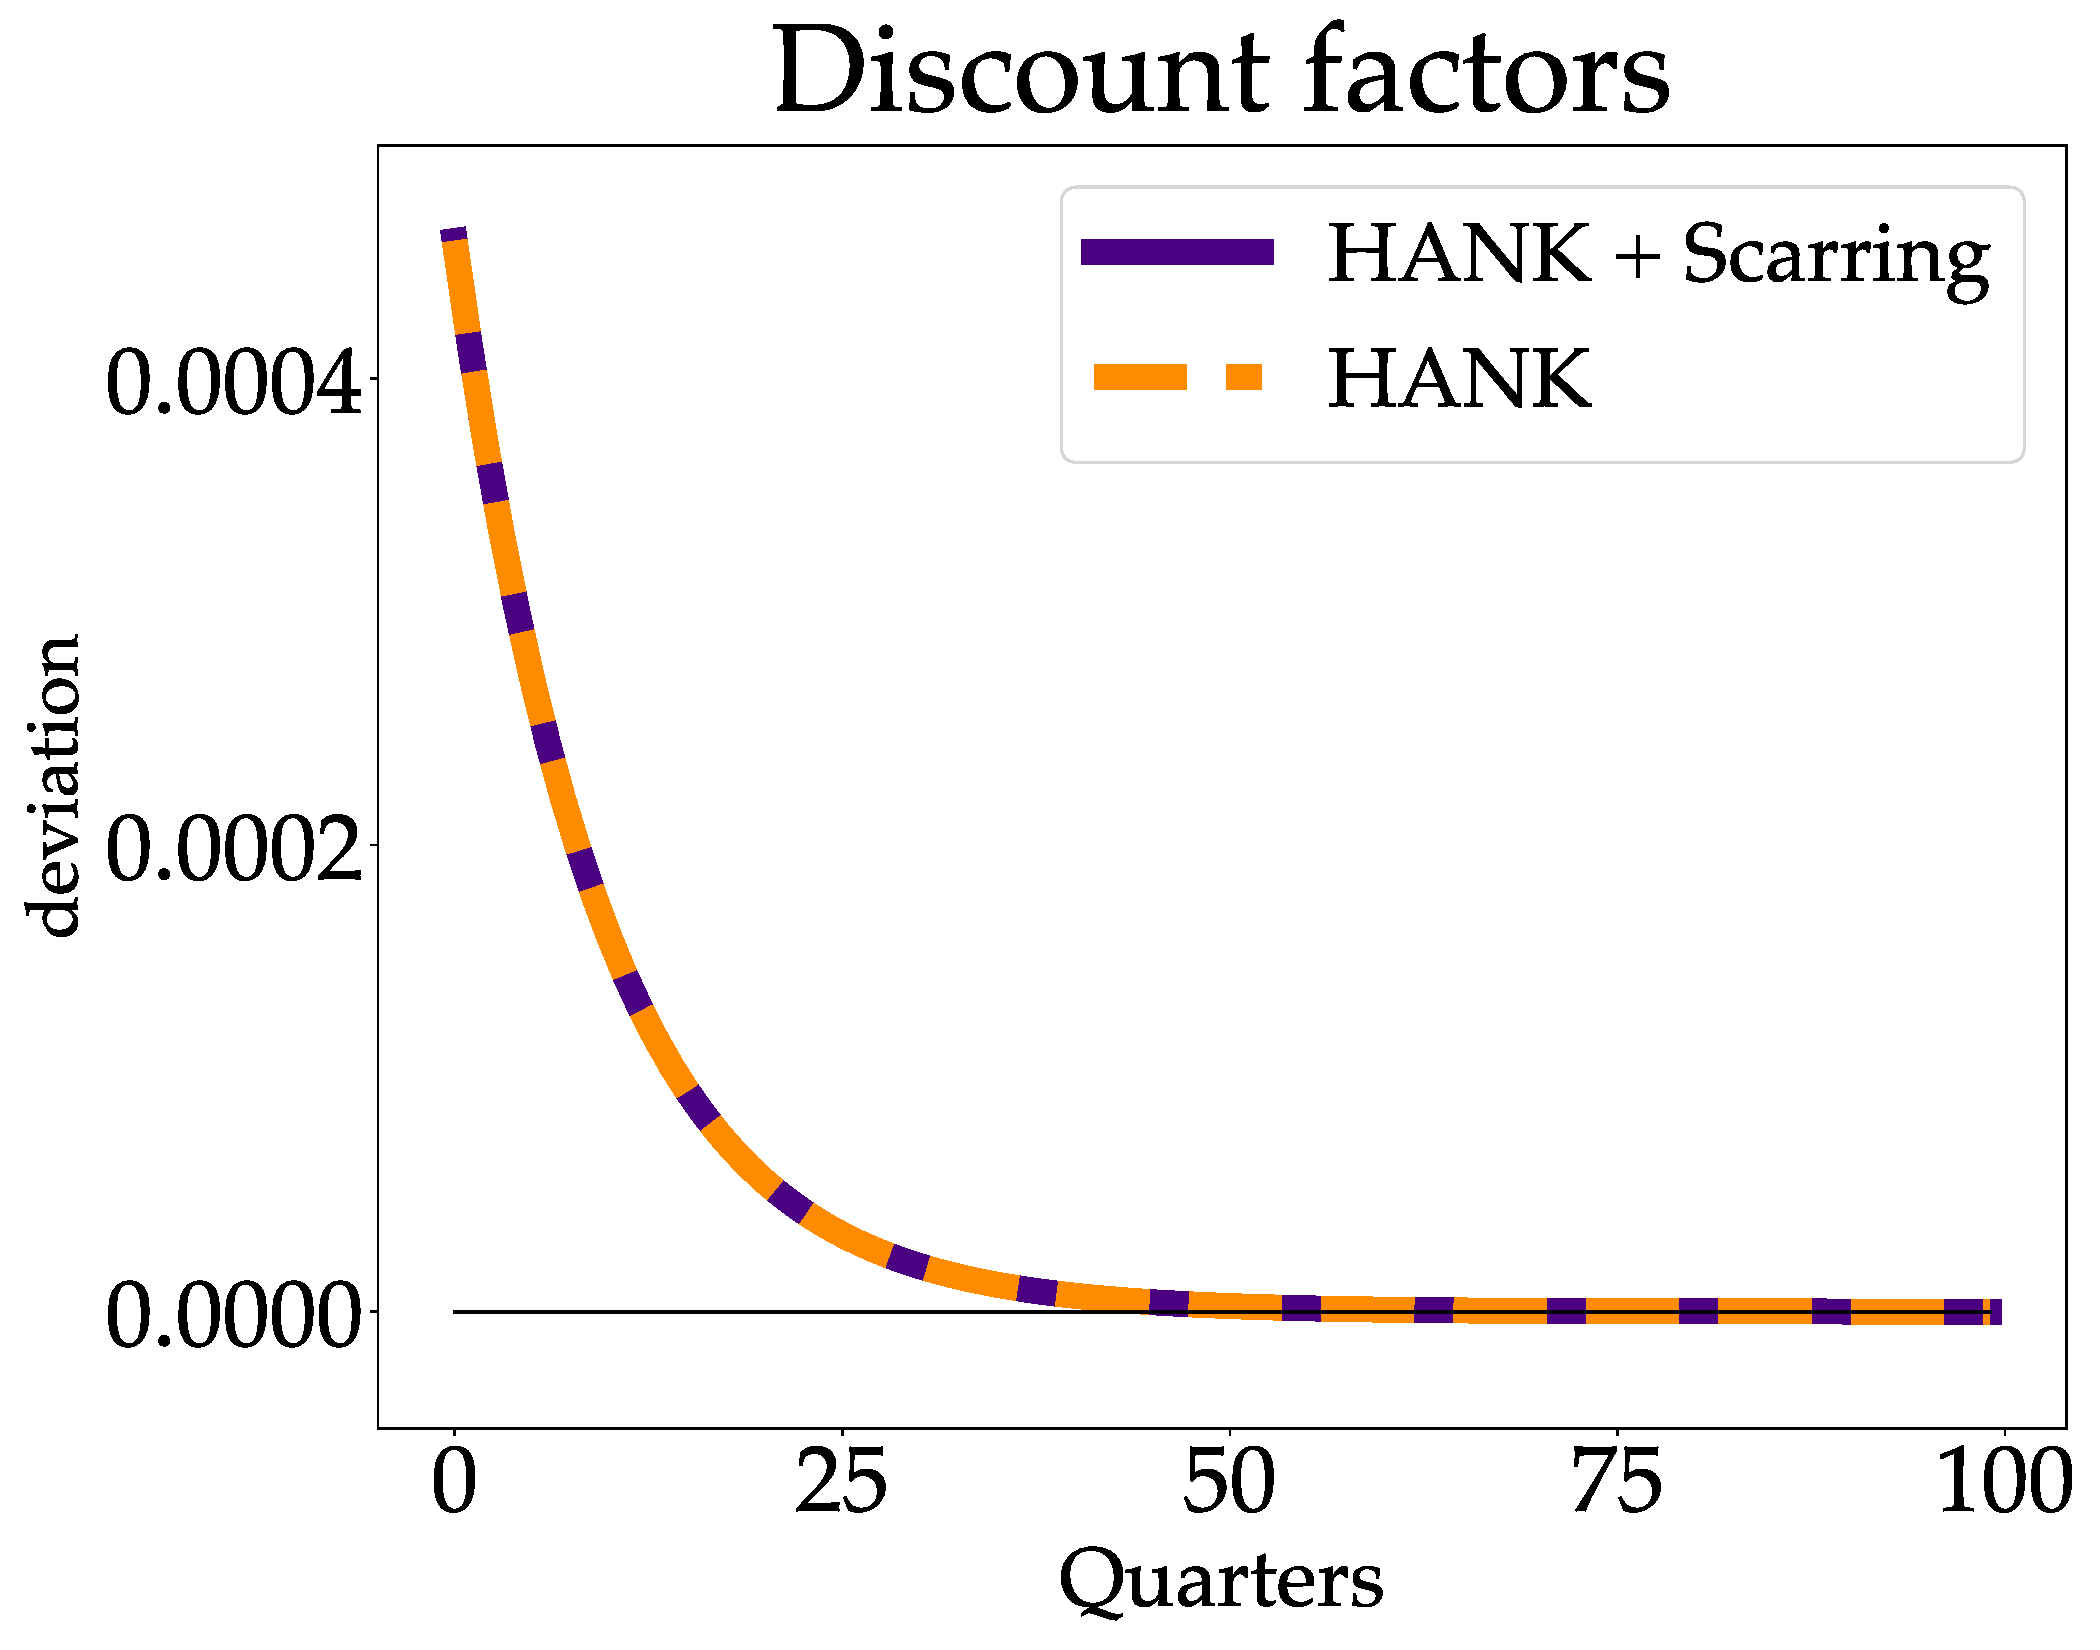
\includegraphics[scale=.14]{text/chapter1/Figures/DiscFac_IPR}
  \label{fig:1}
\end{minipage}\hfil % <-- added
\begin{minipage}{0.33\textwidth}
  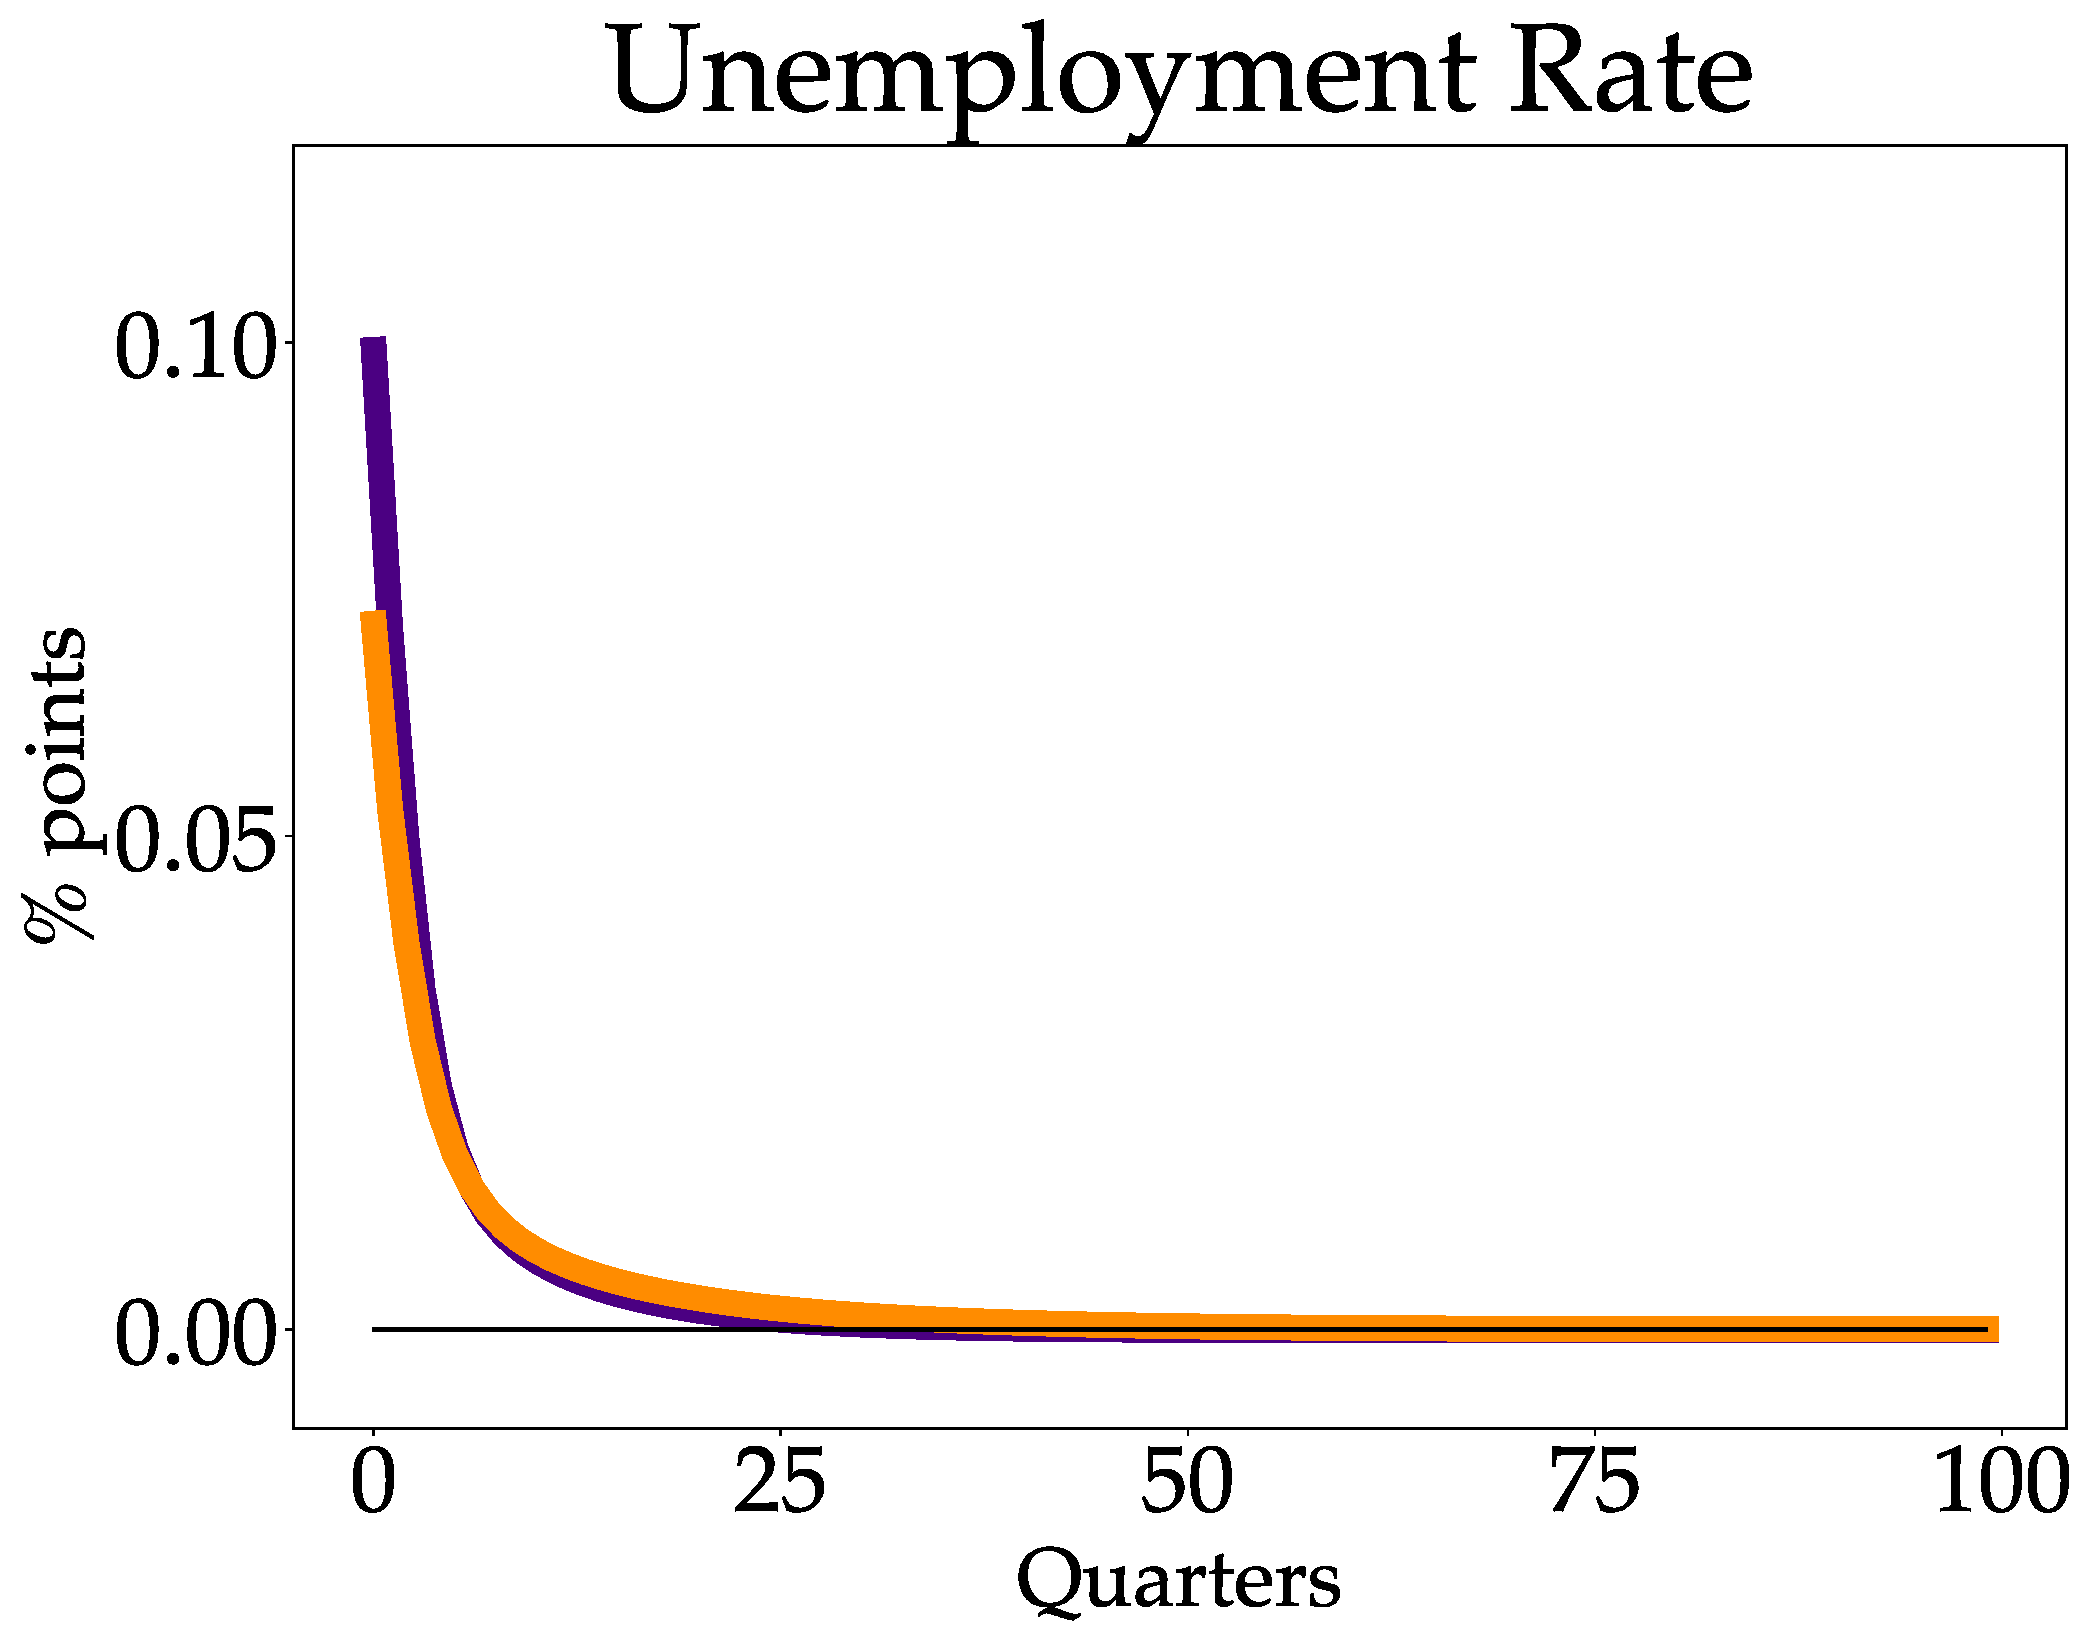
\includegraphics[scale=.14]{text/chapter1/Figures/U_IPR}
  \label{fig:2}
\end{minipage}\hfil % <-- added
\begin{minipage}{0.33\textwidth}
  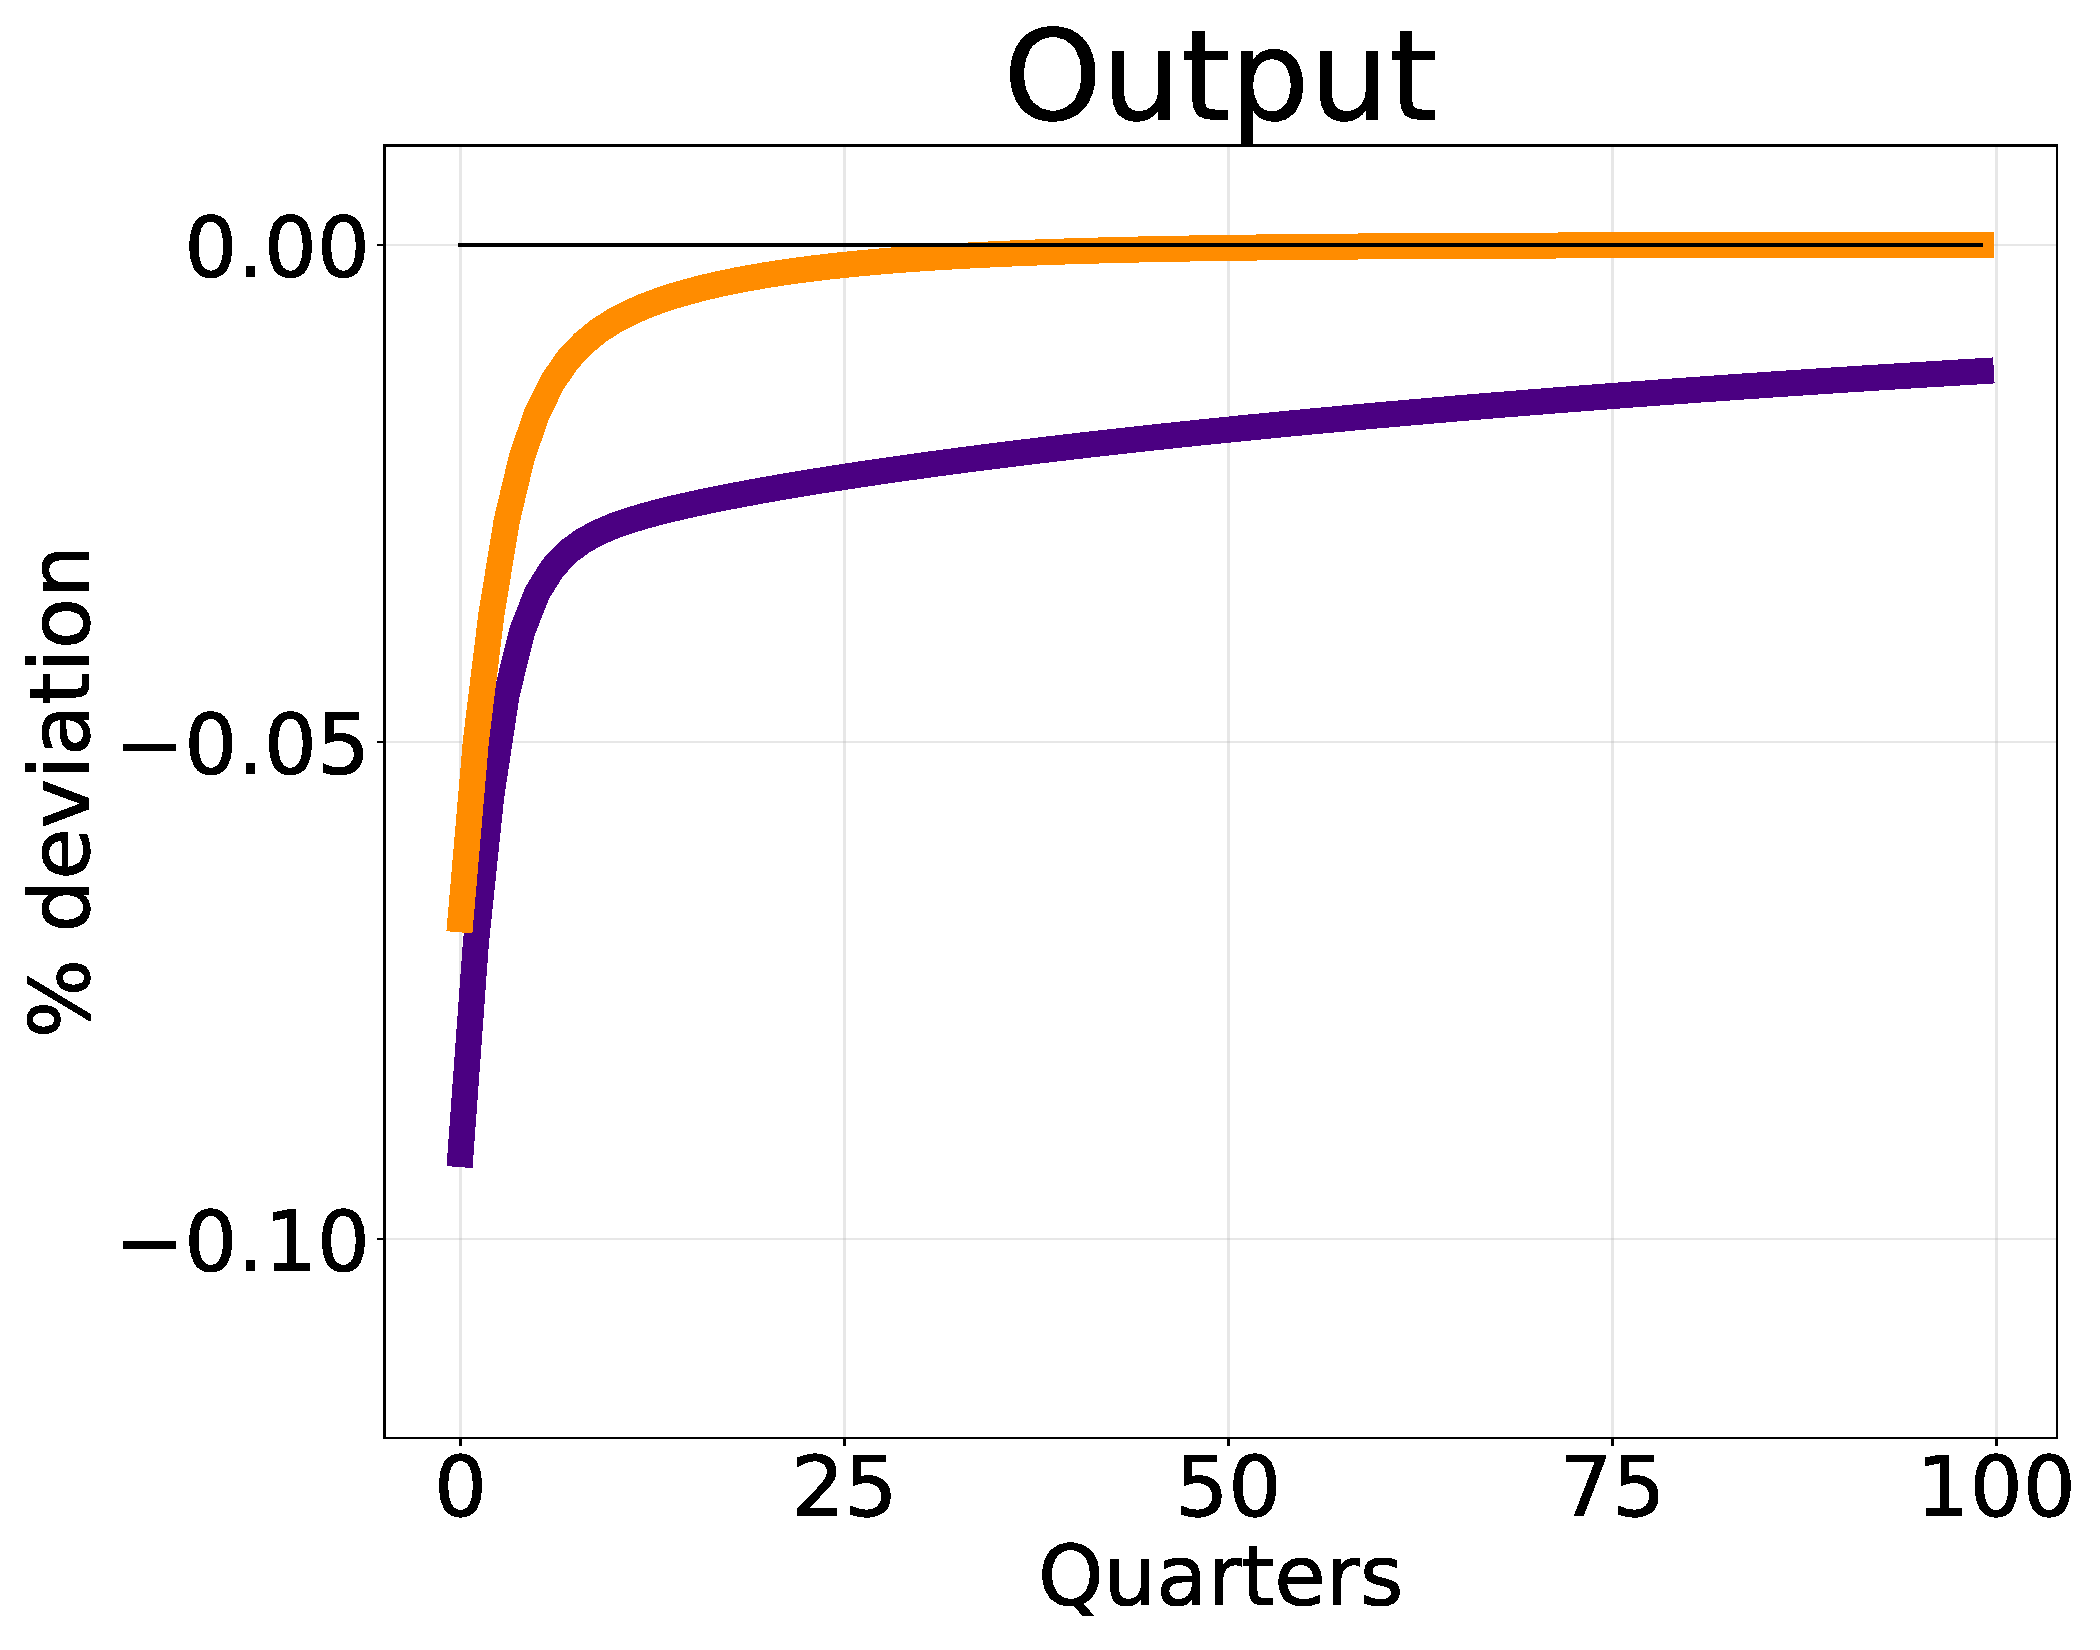
\includegraphics[scale=.14]{text/chapter1/Figures/Y_IPR}
  \label{fig:3}
\end{minipage}
\begin{minipage}{0.33\textwidth}
  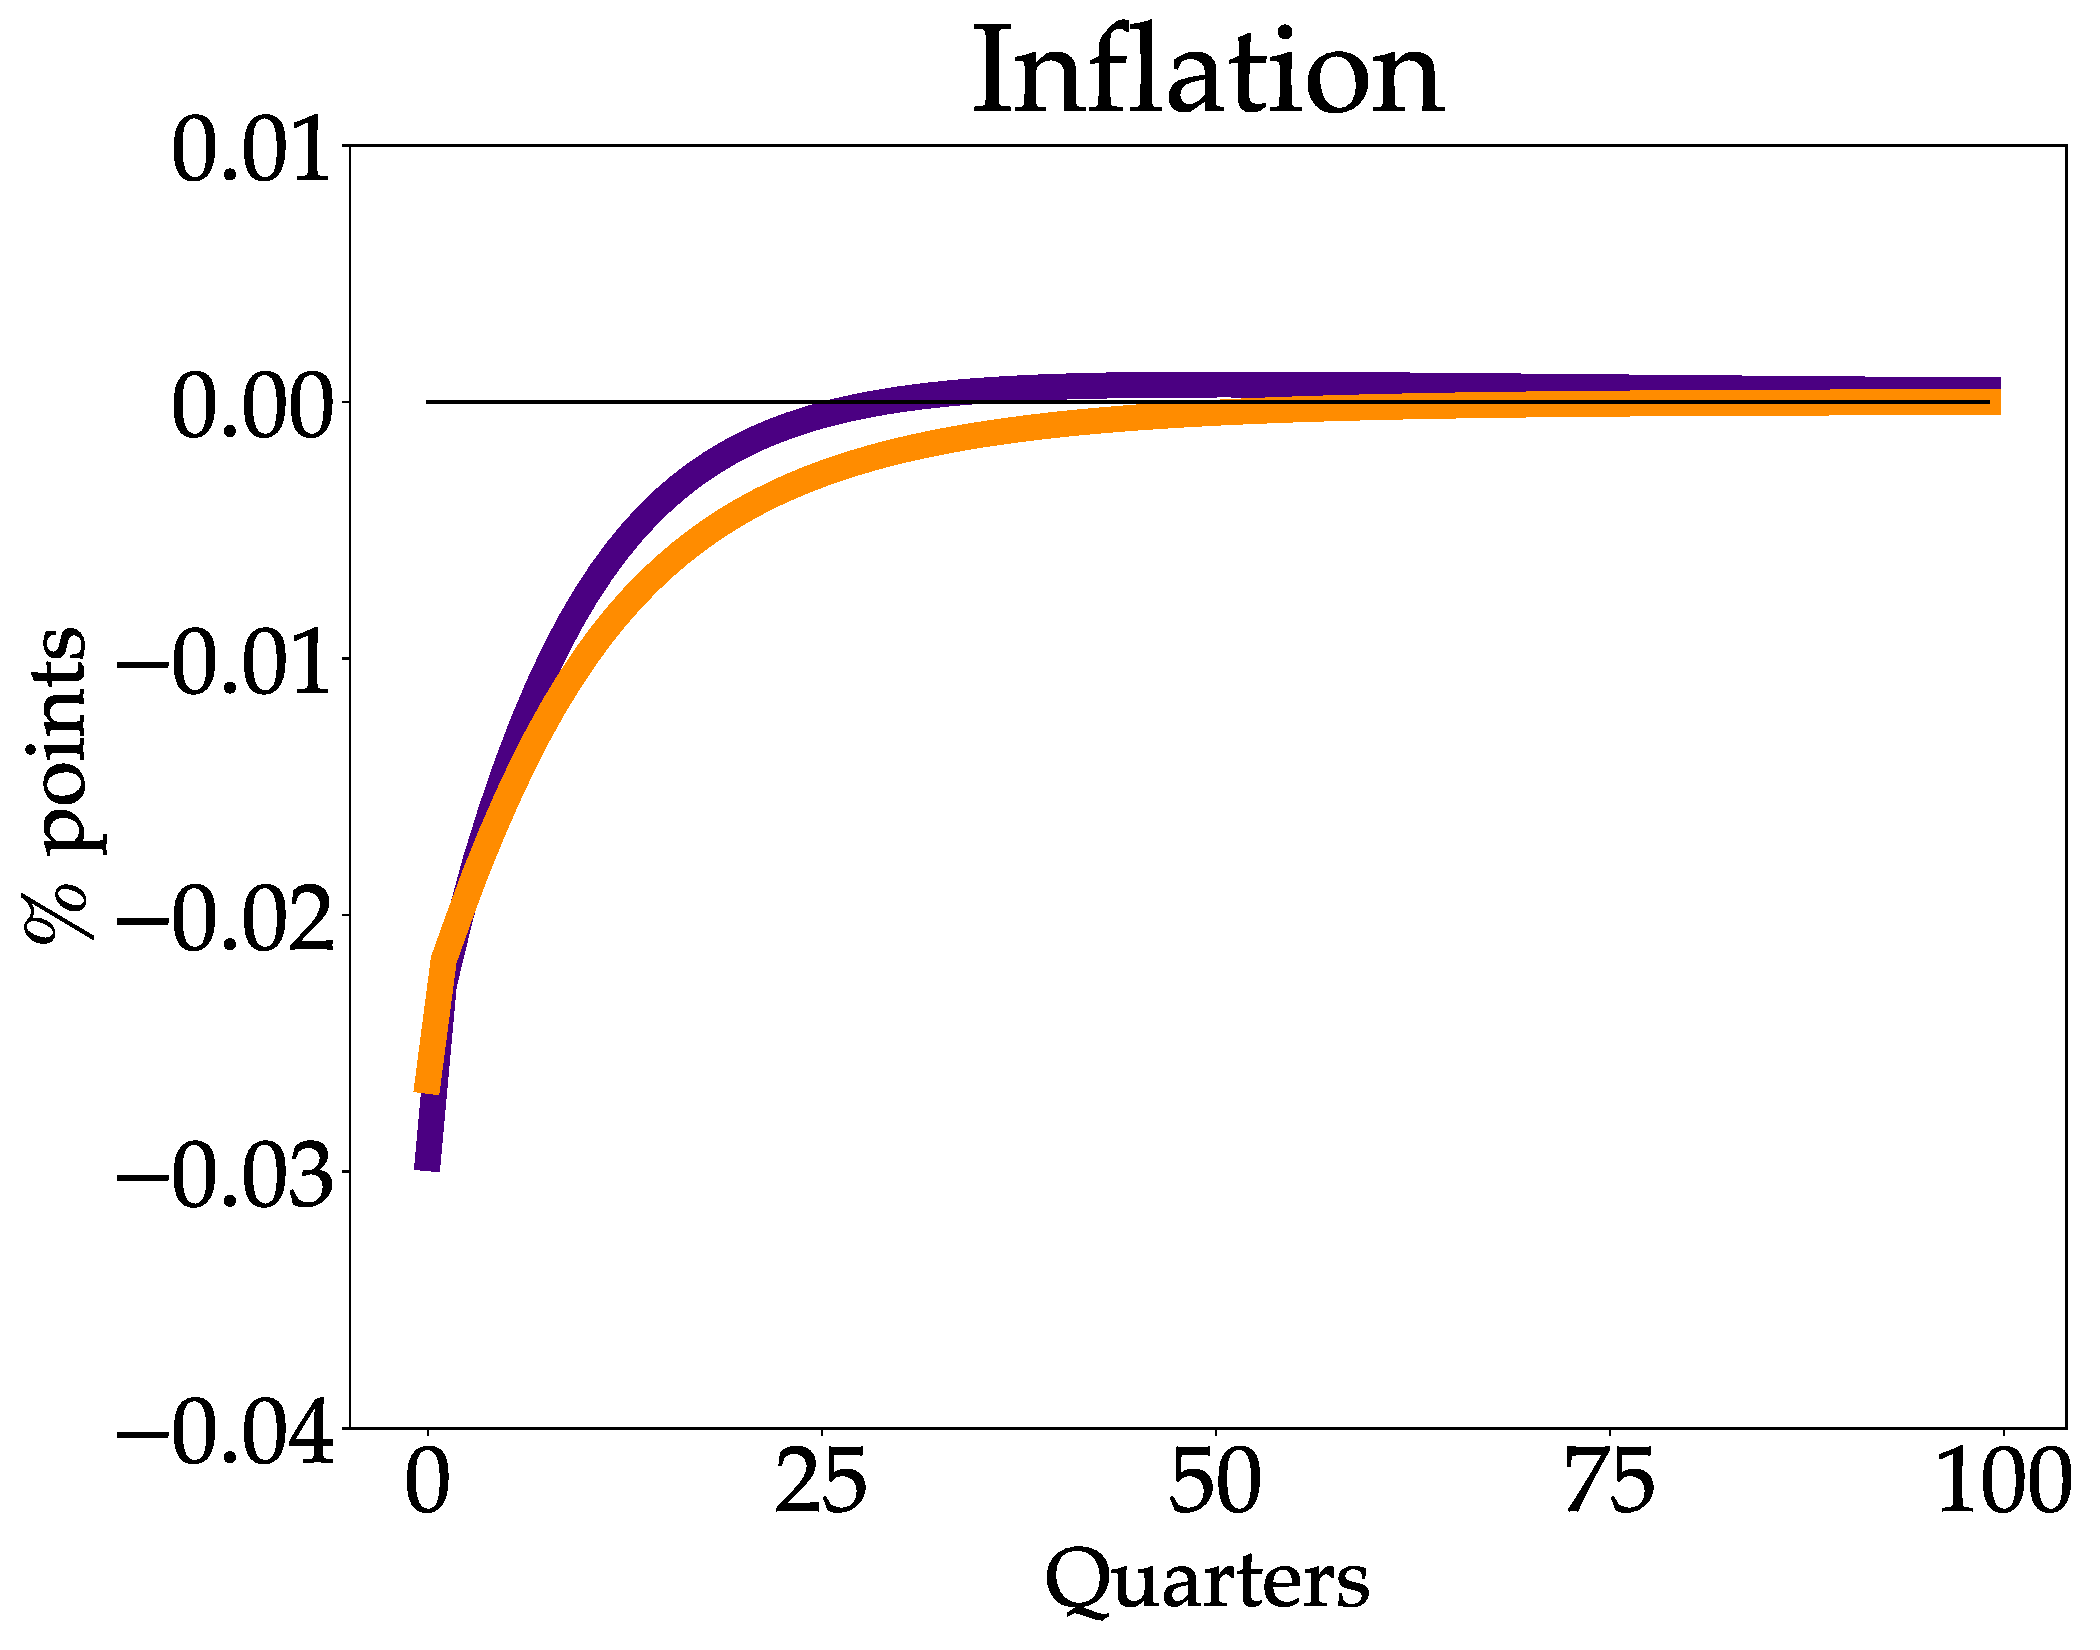
\includegraphics[scale=.14]{text/chapter1/Figures/pi_IPR}
  \label{fig:4}
\end{minipage}
\medskip
\begin{minipage}{0.33\textwidth}
  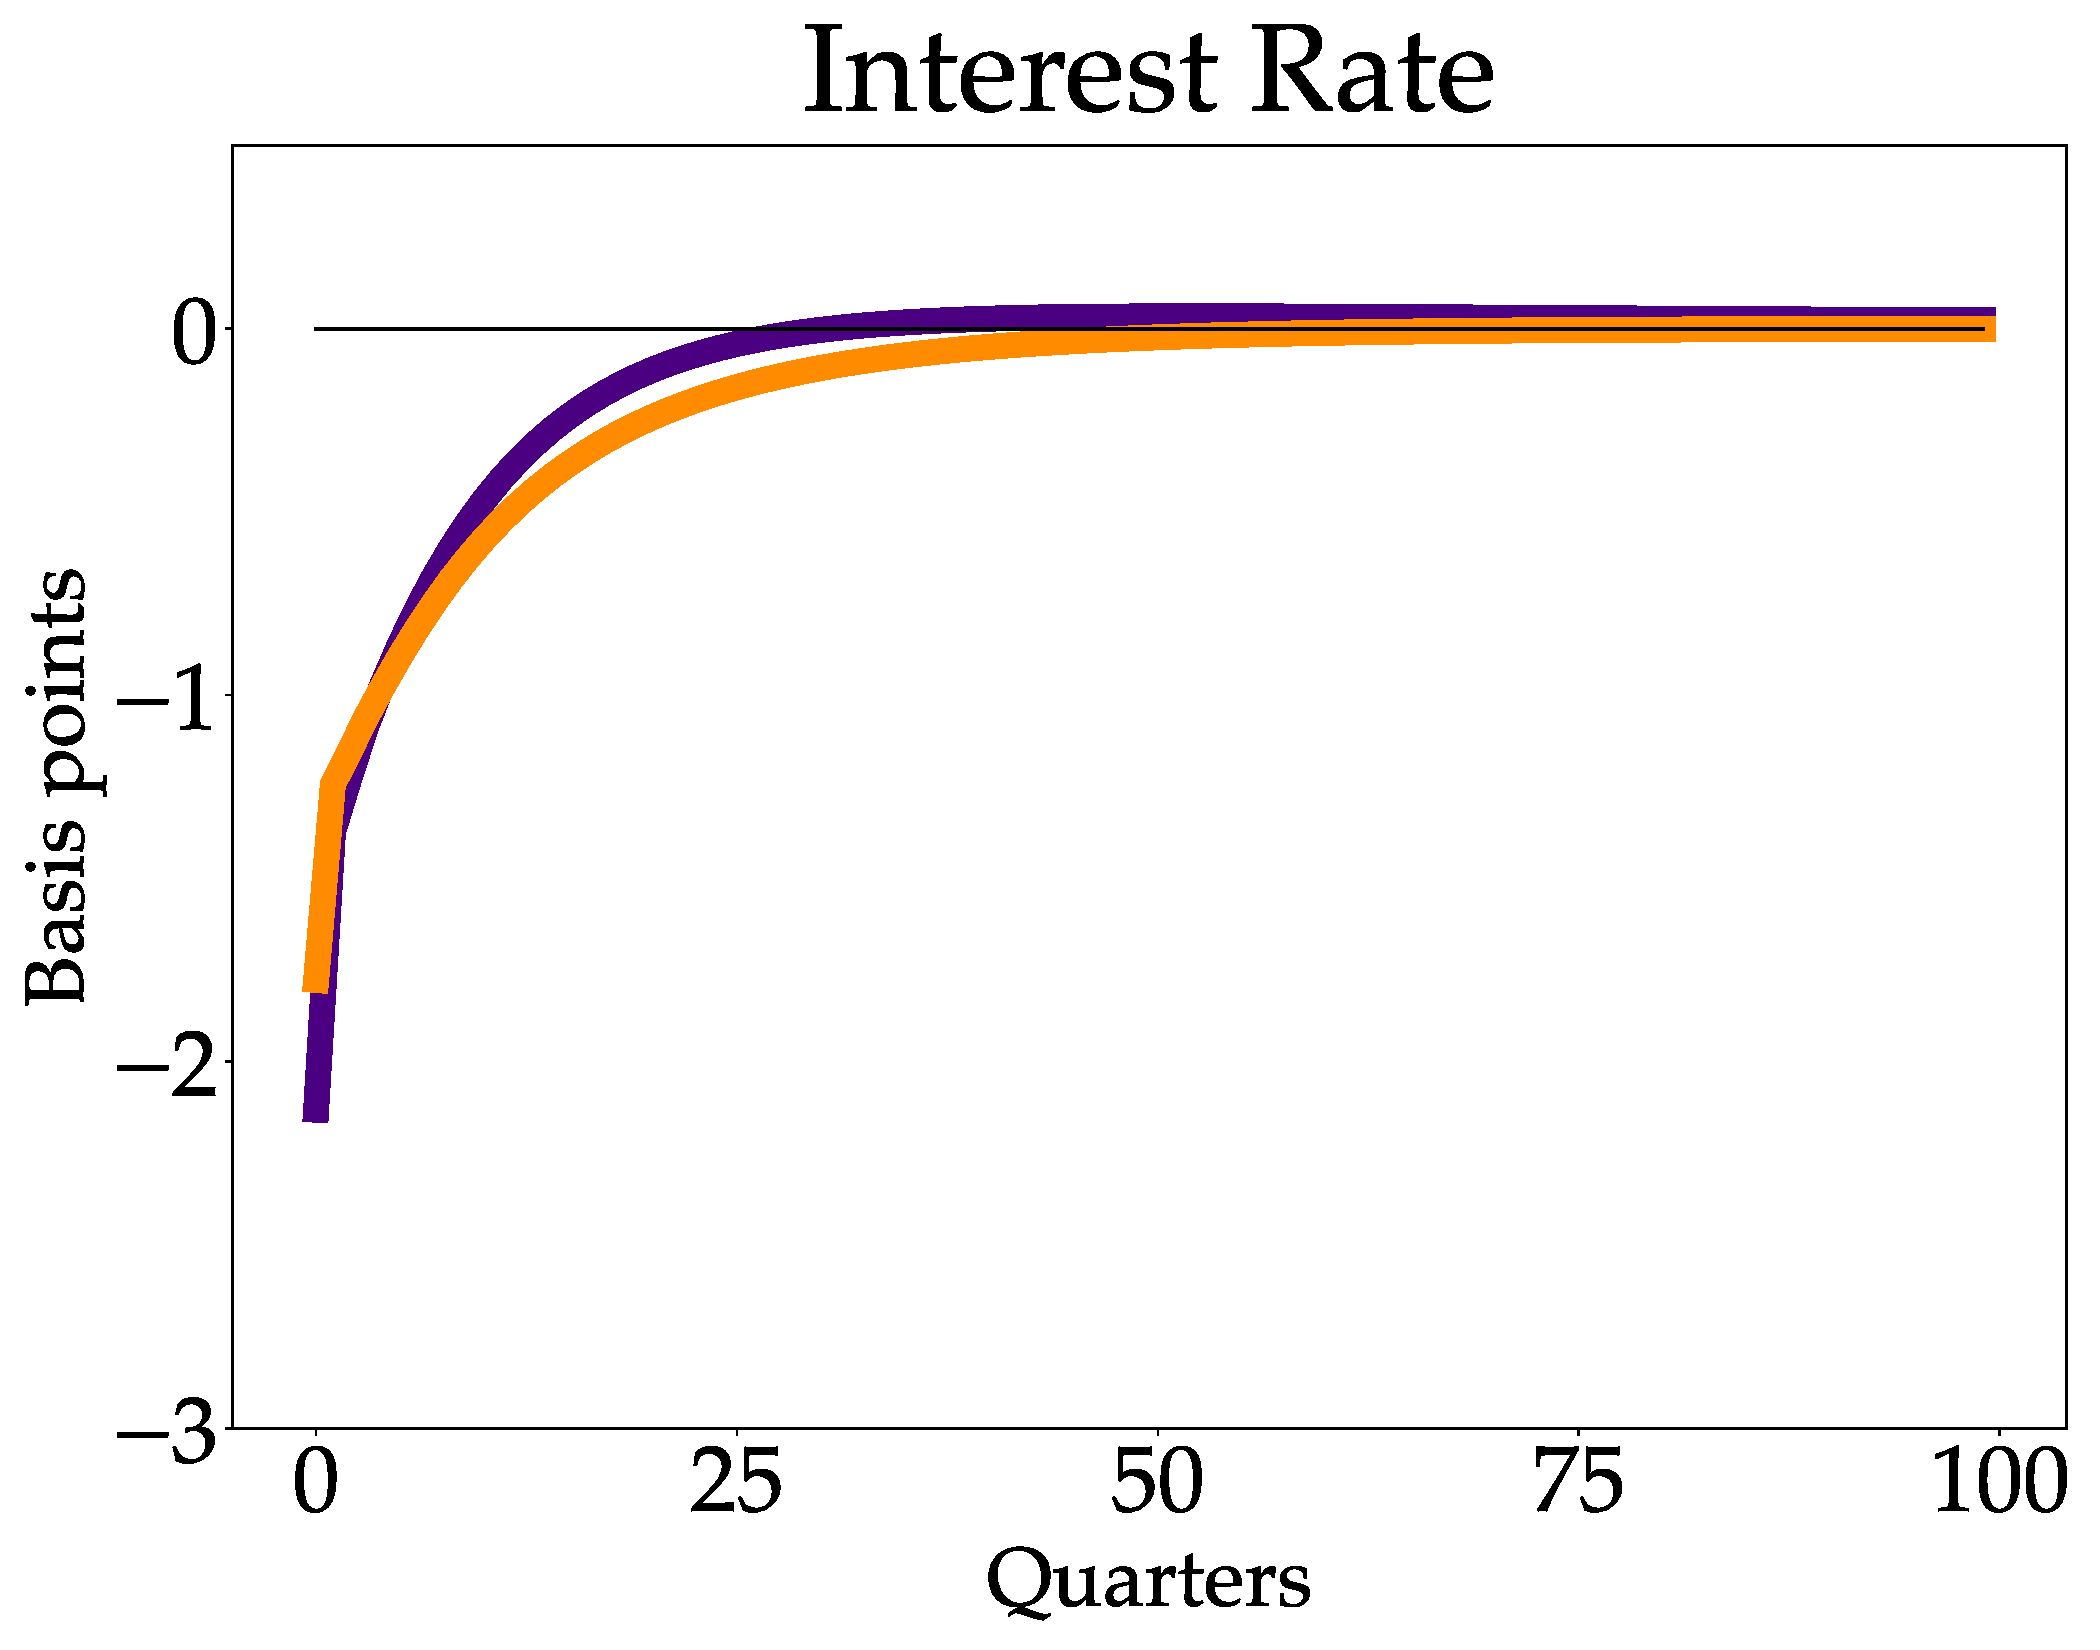
\includegraphics[scale=.14]{text/chapter1/Figures/r_IPR}
  \label{fig:4}
\end{minipage}\hfil % <-- added
\begin{minipage}{0.33\textwidth}
  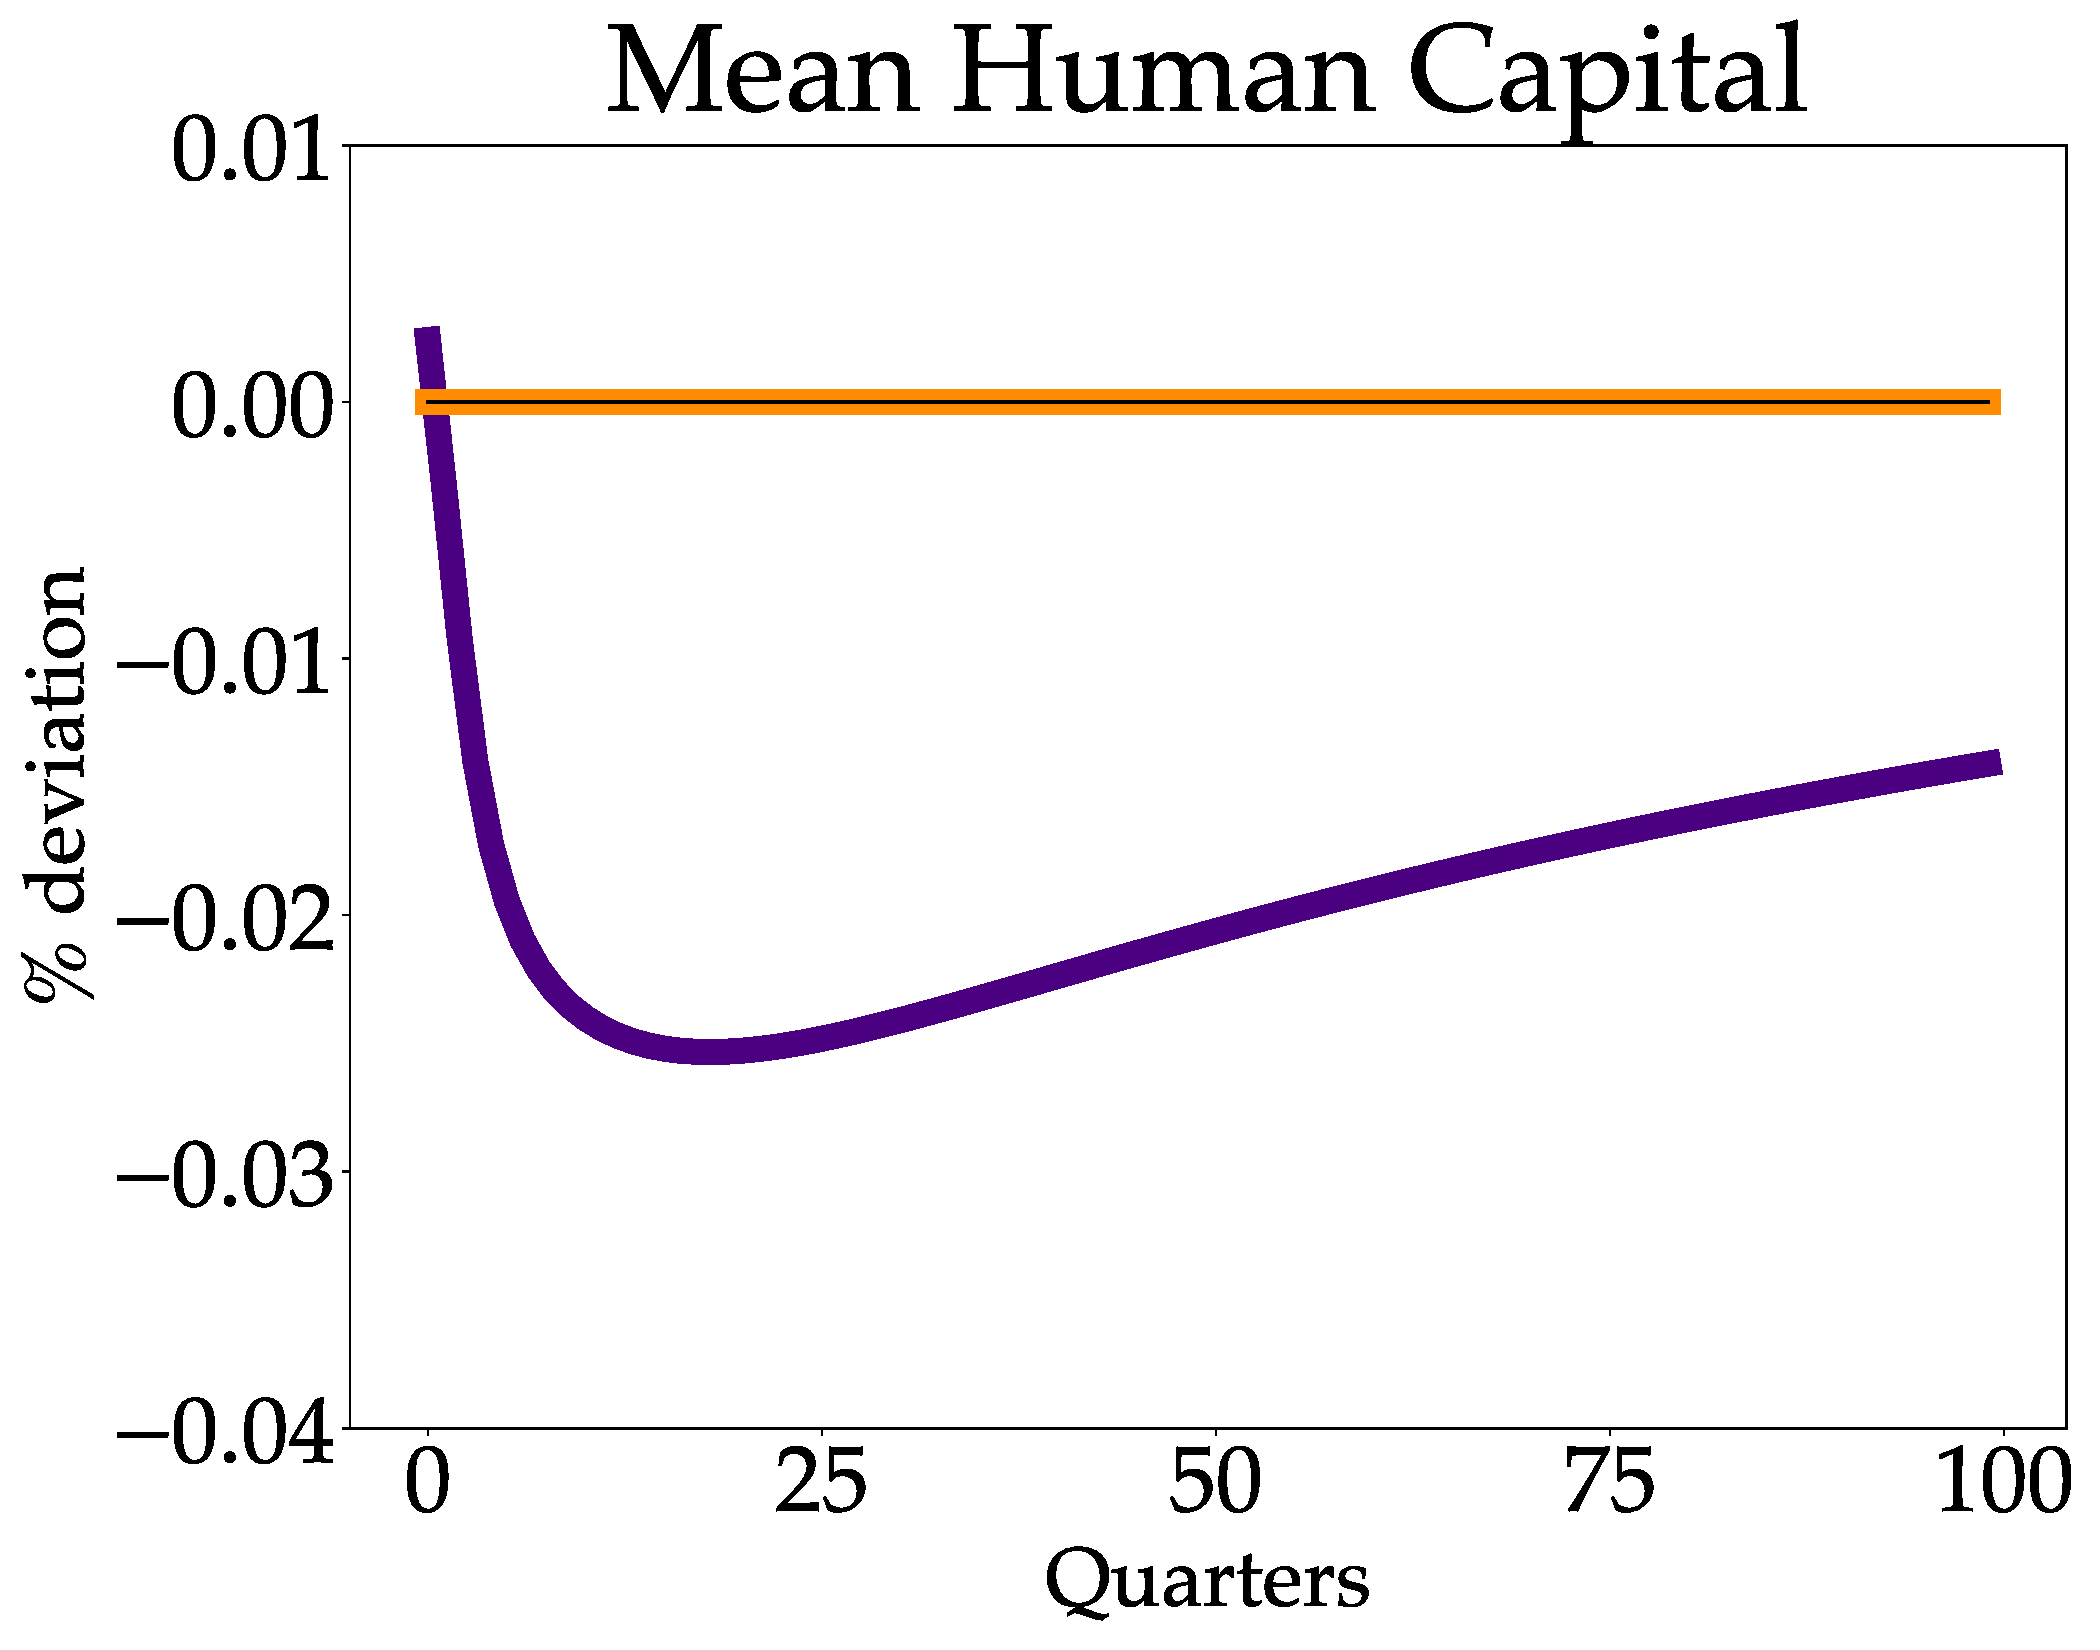
\includegraphics[scale=.14]{text/chapter1/Figures/H_E_IPR}
  \label{fig:5}
\end{minipage}\hfil % <-- added
\caption{Impulse responses to a negative demand shock} 
\floatfoot{Note: The exercise above plots the impulse responses to a positive discount factor shock. The quarterly persistence of the shock is $0.9$ and the size of the shock is then calibrated to generate a 0.1 percentage point increase in the unemployment rate.}
\label{IPR_demand}
\end{figure}


\subsection{Unemployment Scarring and Inequality}

With unemployment scarring, an increase in unemployment leads to a persistent rise in income inequality. Figure \ref{Gini_IPR} plots the impulse response of the labor income gini index across households to the negative demand shock under the baseline model and under the model without scarring. In the baseline model, the initial increase in the gini index is attributed to the rise in unemployment and the decline in the aggregate wage. The persistence of the gini index response is due to the recomposition of the distribution of human capital of employed households. In particular, as unemployed households find reemployment at lower levels of human capital. Since the human capital of newly employed households accumulates slowly, this causes hysteresis in the gini index. In the model without scarring, the increase in income inequality is transitory as it is only affected by transitory changes in the unemployment rate and the aggregate wage.

\begin{figure}[!ht]
   \begin{center}
   \begin{minipage}{0.7\textwidth}
        \centering
        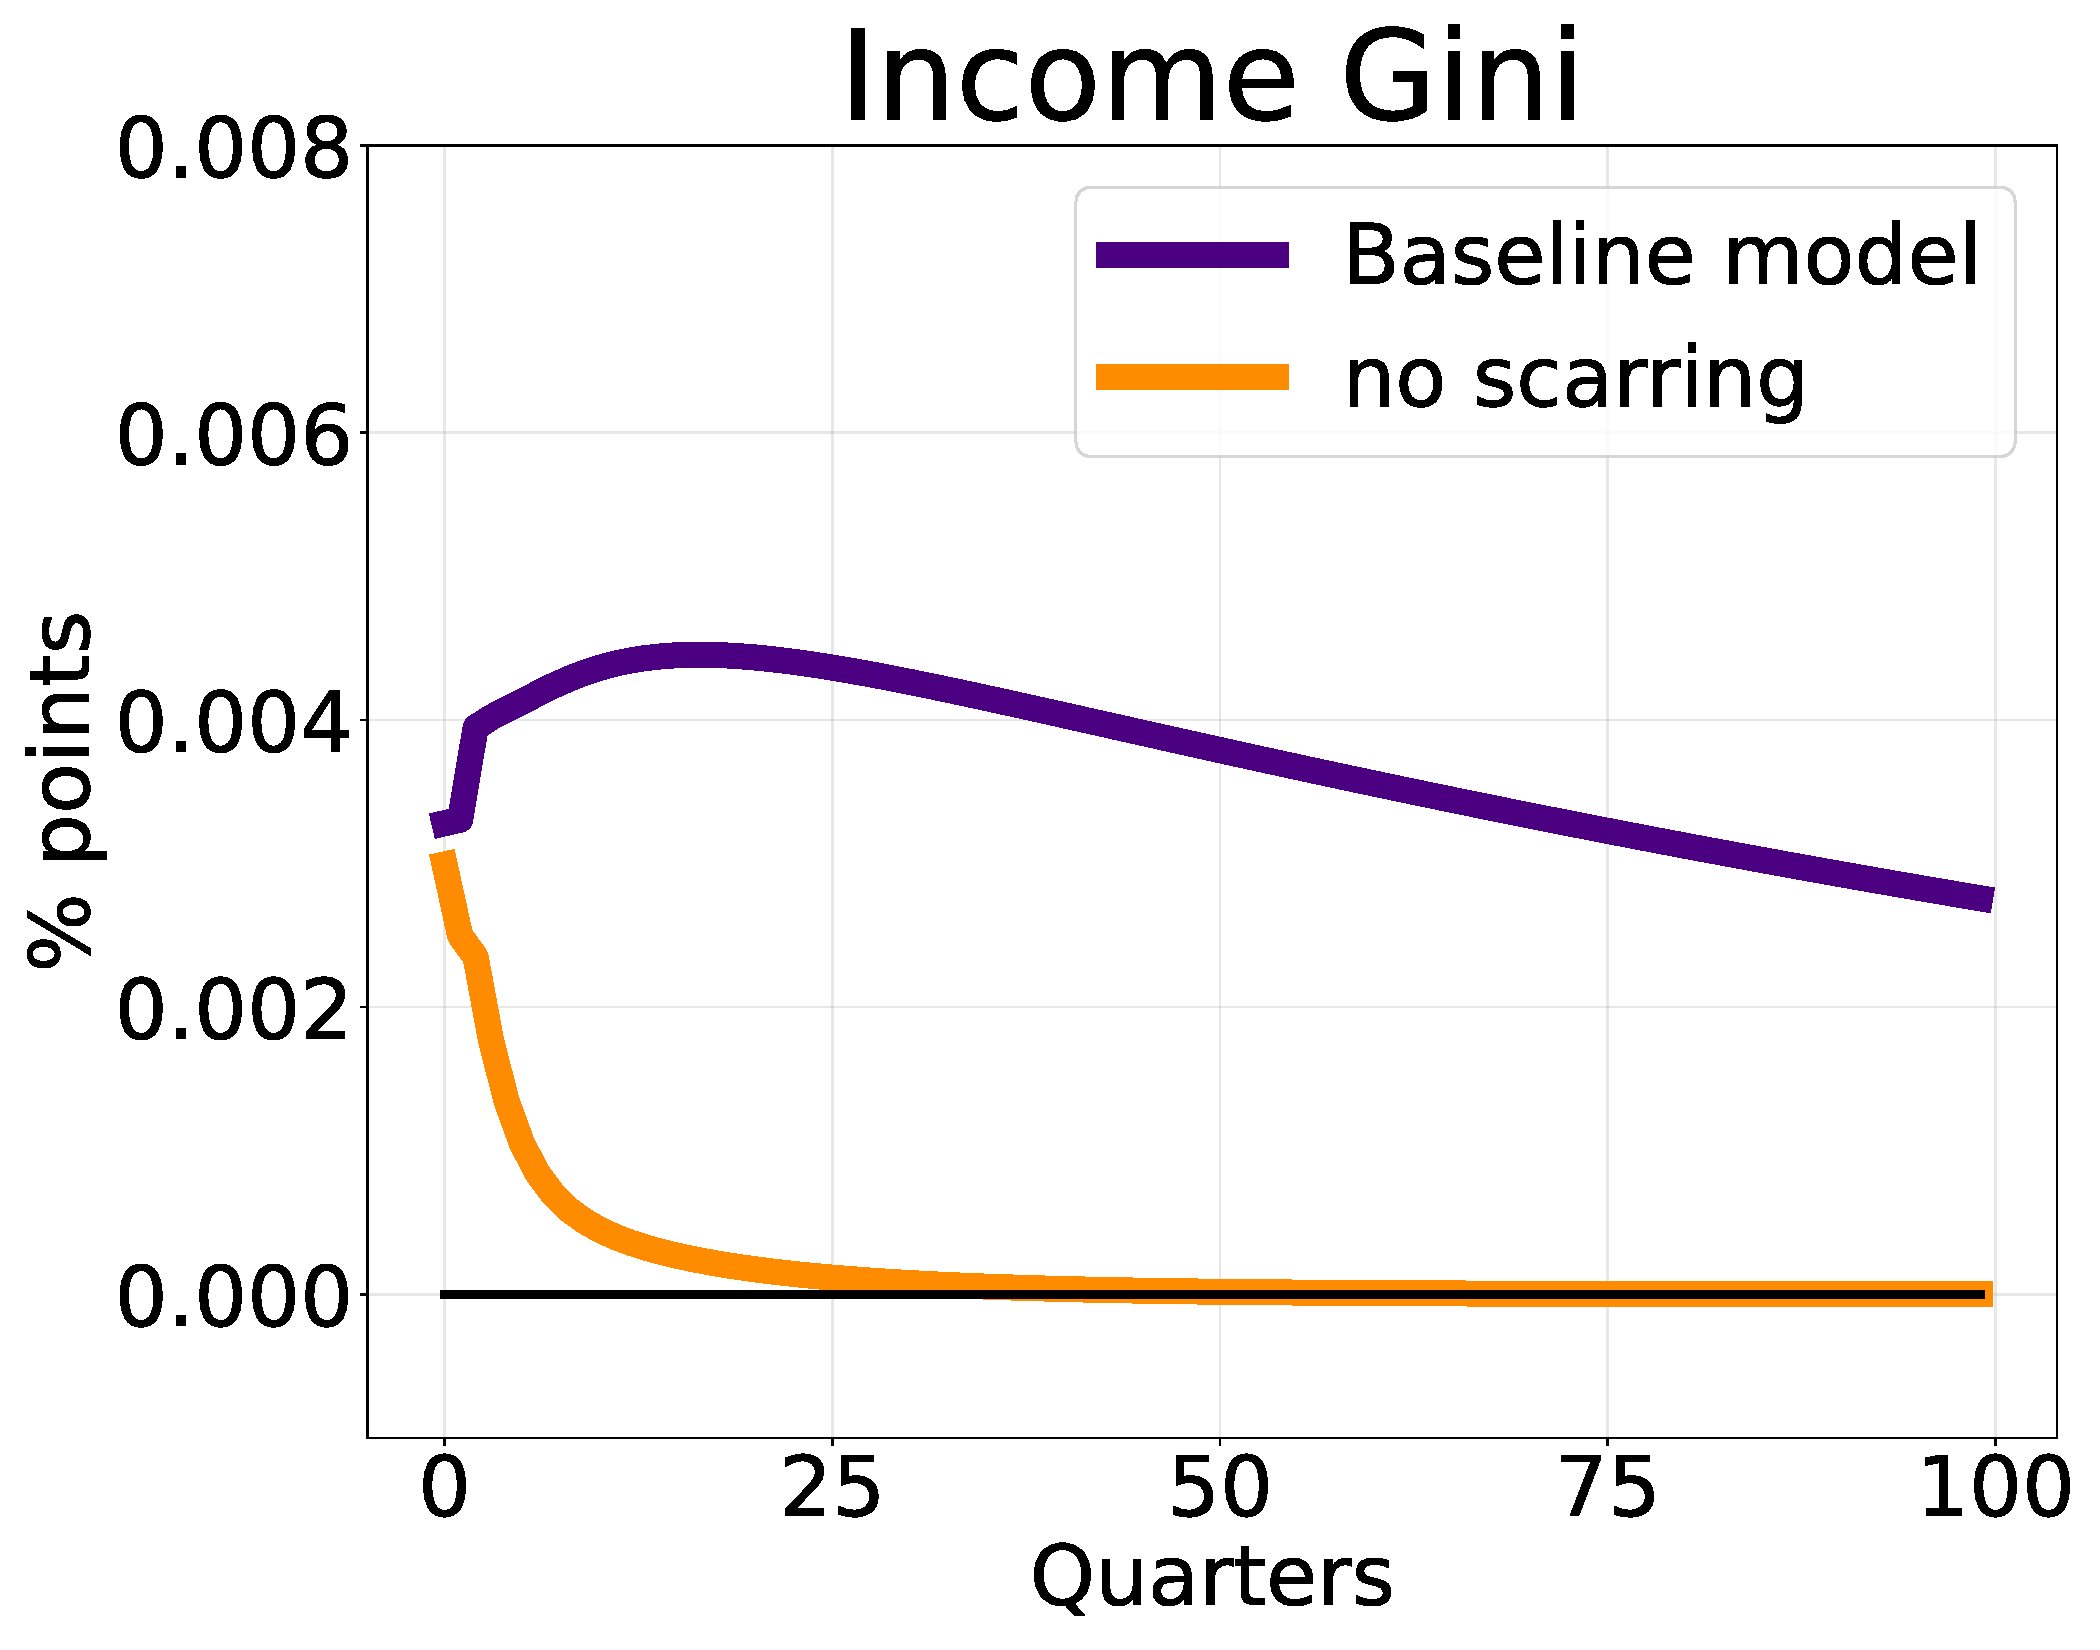
\includegraphics[scale=.3]{text/chapter1/Figures/gini_IPR} % first figure itself
    \end{minipage}
        \caption{Response of income Gini index to negative demand shock.}
        \floatfoot{Note: This exercise plots the impulse response of the Gini index from the negative demand shock in \ref{IPR_demand}.}
    \label{Gini_IPR}
    \end{center}
  \end{figure}




\subsection{Scarring and Debt to GDP}

Unemployment scarring increases the pressure that recessions place on national debt. Figure \ref{debt_to_GDP} plots the responses of debt to GDP and debt to the demand shock from previous section. The figure demonstrates that the debt to GDP and debt increase much more persistently in the presence of scarring. This is due to the pressure that scarring places on tax revenues. As households lose their jobs and find reemployment at a lower effective wage, the tax base is scarred. This persistent decline in tax revenues require the government to borrow substantially more to maintain their expenditures.


\begin{figure}[!ht]
    \centering
   \begin{minipage}{0.47\textwidth}
        \centering
        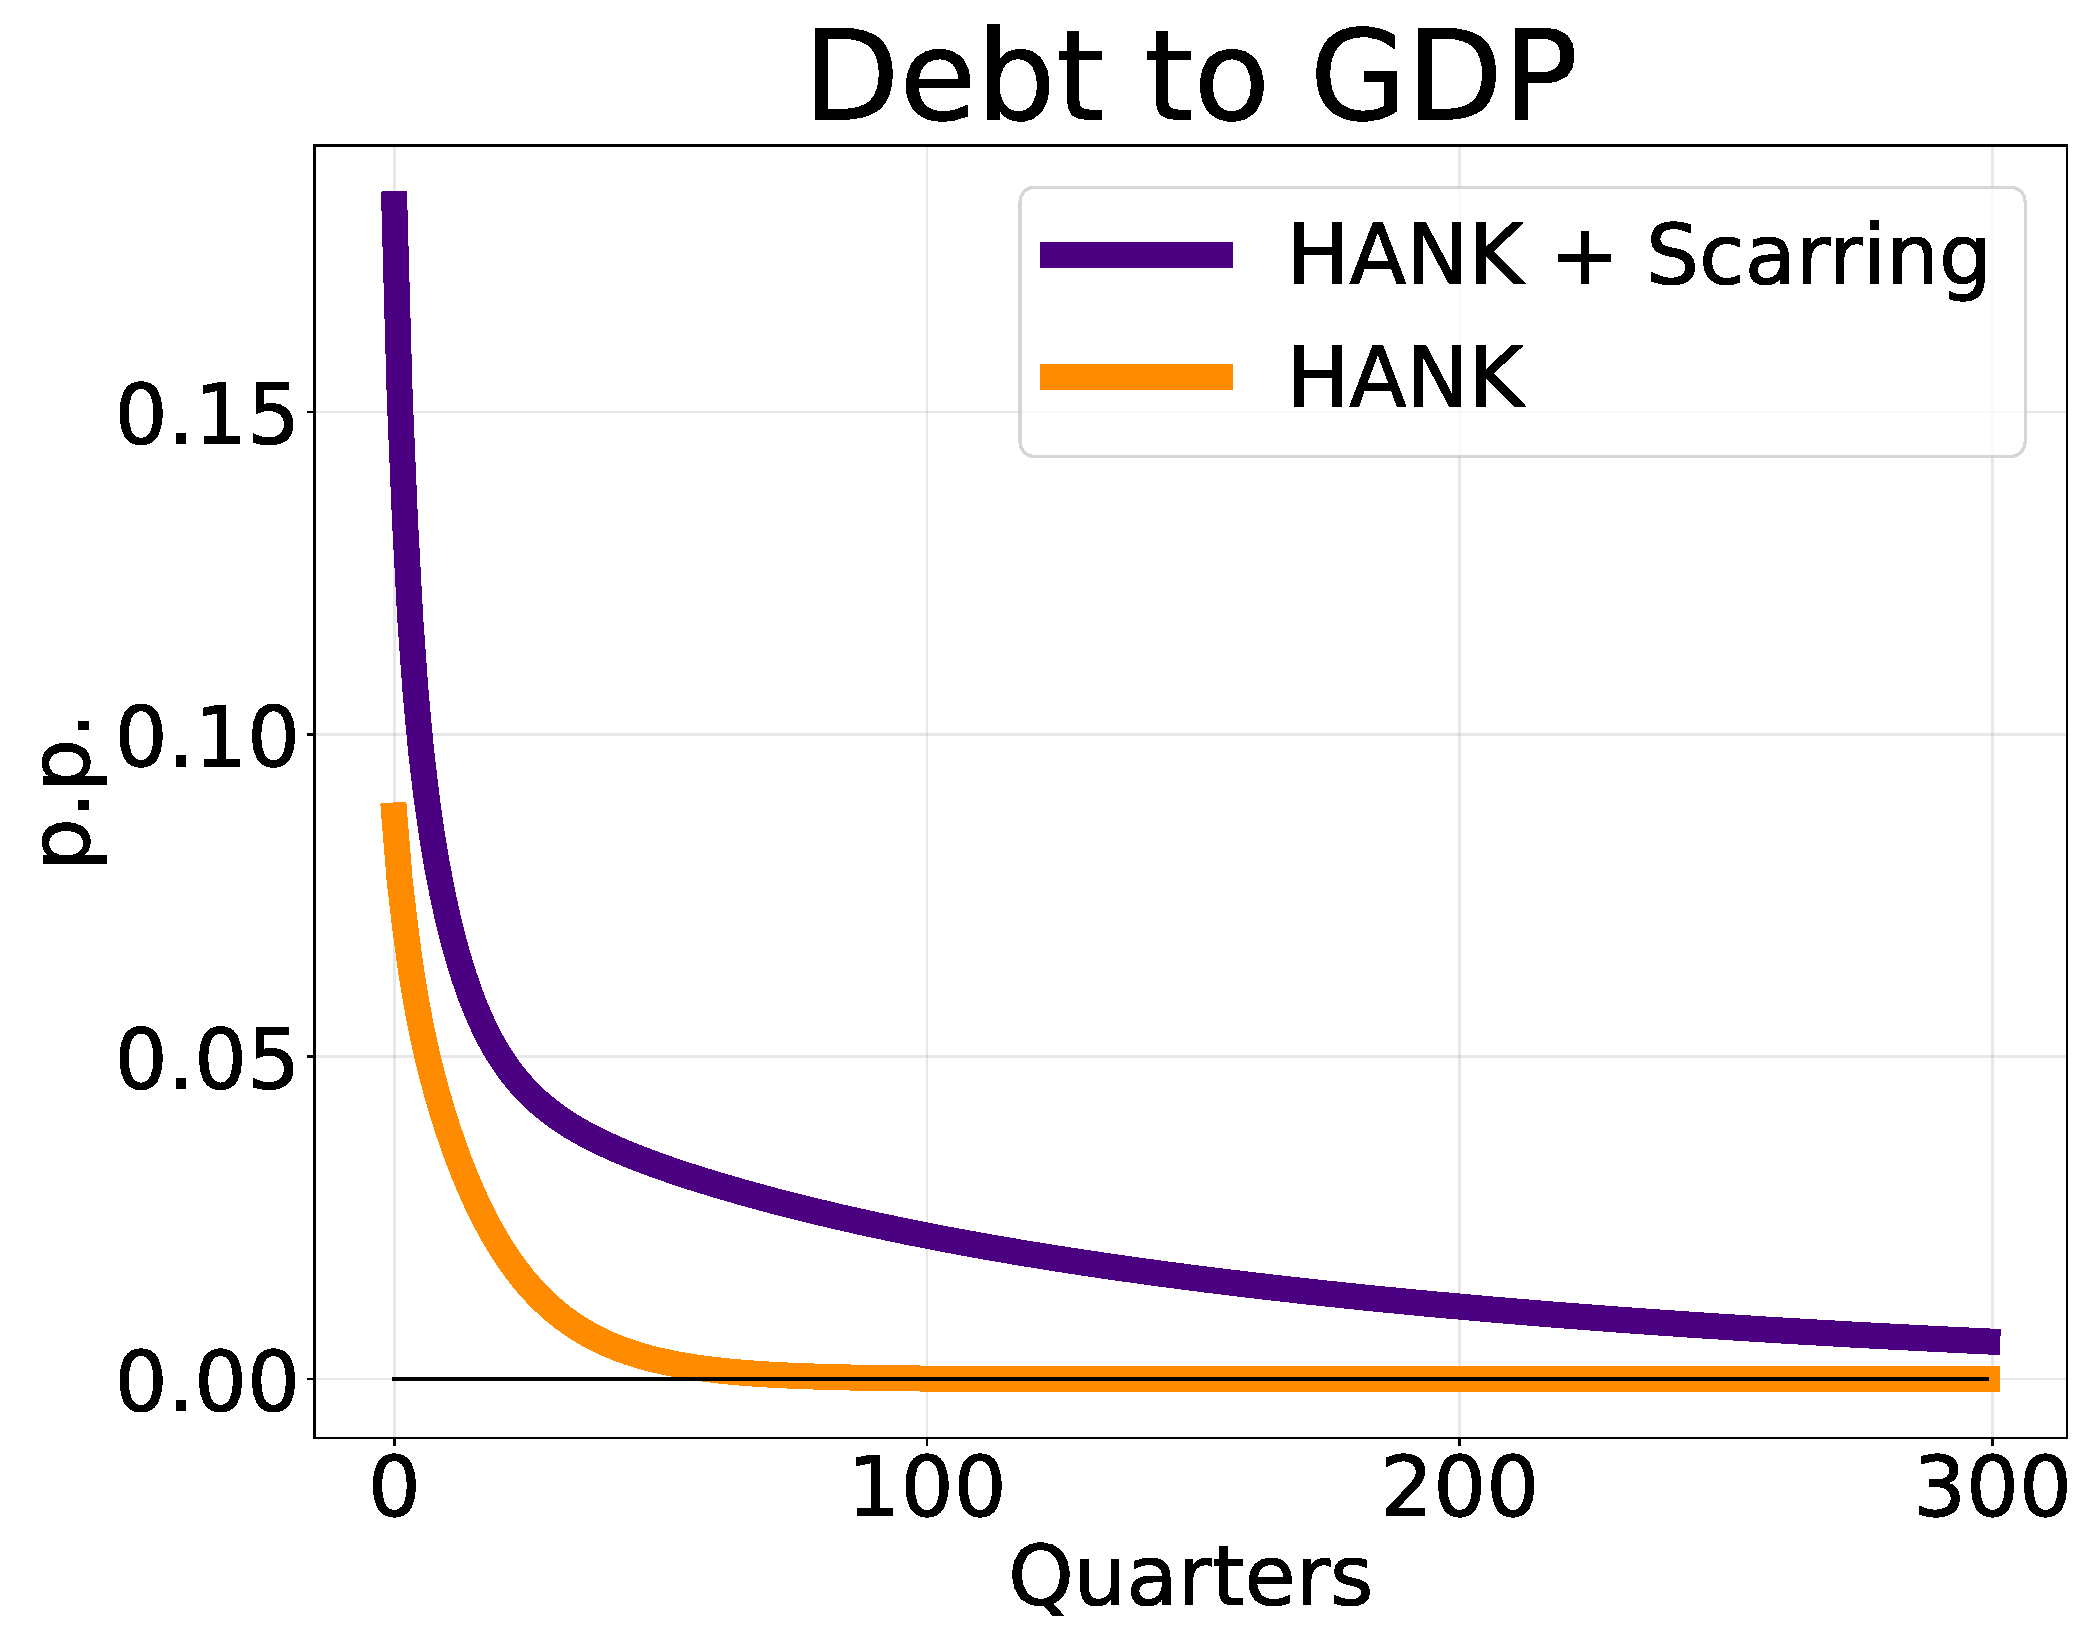
\includegraphics[scale=.2]{text/chapter1/Figures/debt_to_GDP_IPR} % first figure itself
    \end{minipage}\hfill
    \begin{minipage}{0.47\textwidth}
        \centering
        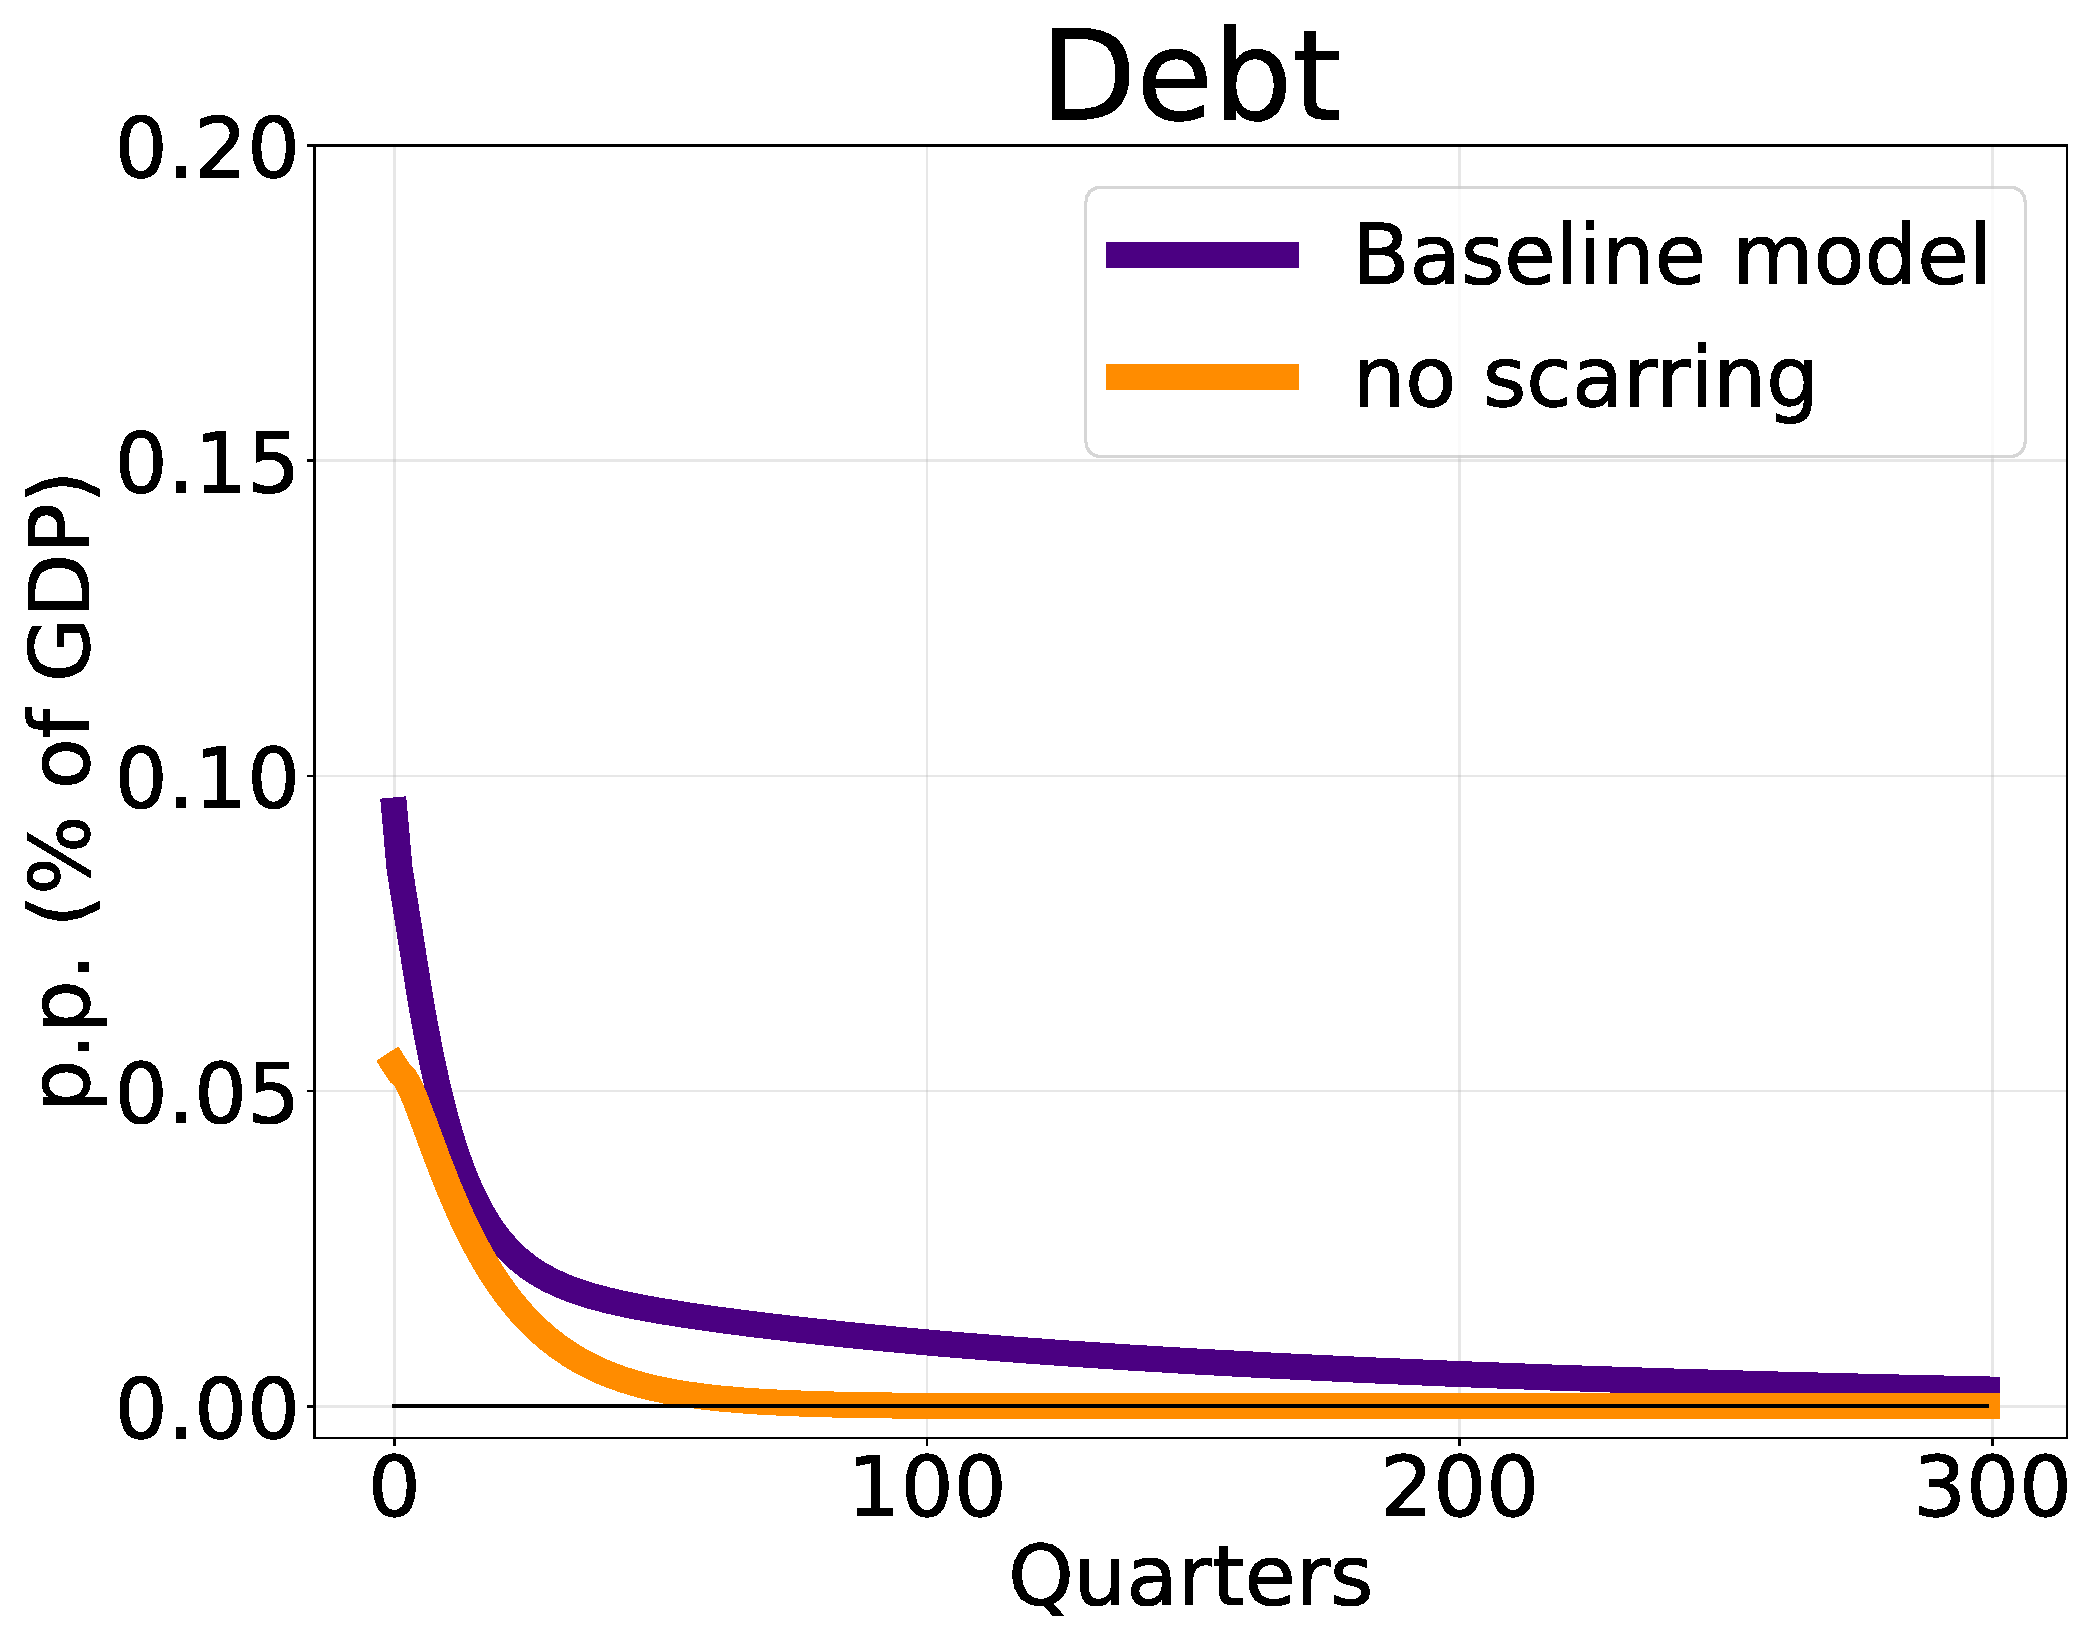
\includegraphics[scale=.2]{text/chapter1/Figures/debt_IPR} % second figure itself
    \end{minipage}
    \caption{Responses of debt and debt to GDP to negative demand shock}
     \floatfoot{Note: This exercise plots response of the debt-to-GDP and debt from the negative demand shock in \ref{IPR_demand}.}
    \label{debt_to_GDP}
\end{figure}


\section{Scarring and the Transmission of Fiscal Policy}


\hypertarget{Fiscal Multipliers}{}
\subsection{Fiscal Multipliers}

Having established that in the presence of unemployment scarring, aggregate shocks lead to persistent responses in output. In this section, I show that fiscal multipliers are substantially larger and rise with the horizon because of unemployment scarring. To do so, I consider a negative government spending shock in the baseline model and the model without scarring and compute the multipliers across the horizon. In particular the multiplier is defined as:



$$ \text{Multiplier} = \frac{\Sigma_{t=0}^{H}  \frac{1}{R^{t}}\Delta Y_{t}}{ \Sigma_{t=0}^{H}  \frac{1}{R^{t}}\Delta{G_{t}}}$$ 

where $H$ is the horizon of the mulitplier. \\

Figure \ref{Fiscal_multipliers} plots the fiscal multipliers to a contractionary government spending shock across the horizon of the multiplier under the baseline model and model without scarring.


\begin{figure}[!ht]
    \centering
   \begin{minipage}{0.68\textwidth}
        \centering
        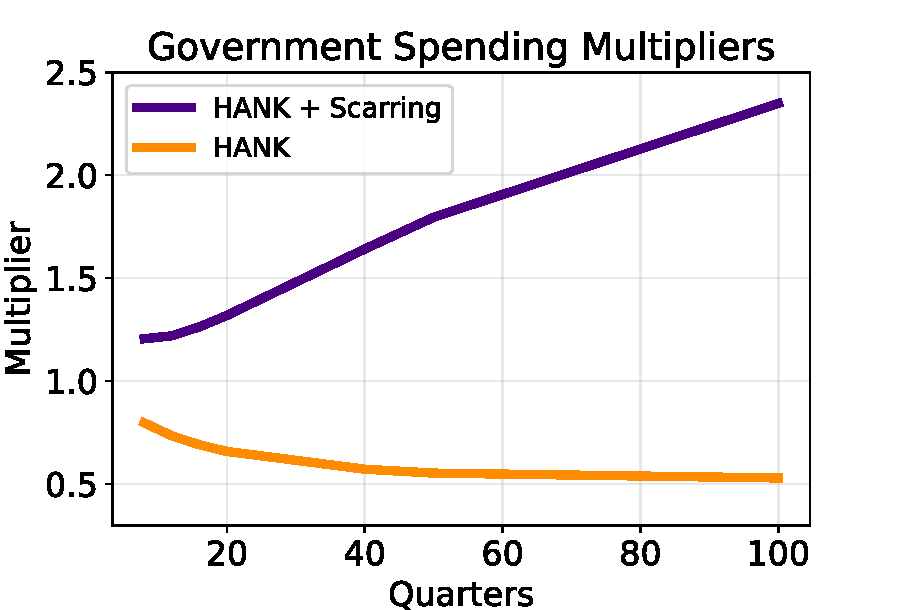
\includegraphics[scale=.7]{text/chapter1/Figures/multipliers} % first figure itself
    \end{minipage}
        \caption{Fiscal Multipliers to a negative government spending shock.}
    \label{Fiscal_multipliers}
    \floatfoot{Note: This figure plots the multiplier out of negative government spending shock with a quarterly AR(1) persistence of 0.933 across the horizon $H$ of the multiplier. For example, a point on the purple line at quarters = 20 represents the fiscal multiplier: $ \frac{\Sigma_{t=0}^{20}  \frac{1}{R^{t}}\Delta Y_{t}}{ \Sigma_{t=0}^{20}  \frac{1}{R^{t}}\Delta{G_{t}}}$. }
\end{figure}


The multipliers under the baseline model rise sharply with the horizon while the multipliers in the model without scarring falls gradually with the horizon. This is because unemployment scarring leads the decline in output in response to the fall in government spending to persist long after the government spending shock recovers.














